% Author: Izaak Neutelings (July 2017)
% Timelines & energy scales of particle physics
\documentclass[border=1pt,tikz]{standalone}

\usepackage{amsmath} % for \dfrac
\usepackage{tikz}
\tikzset{>=latex} % for LaTeX arrow head

\begin{document}


% TIMELINE - simple test
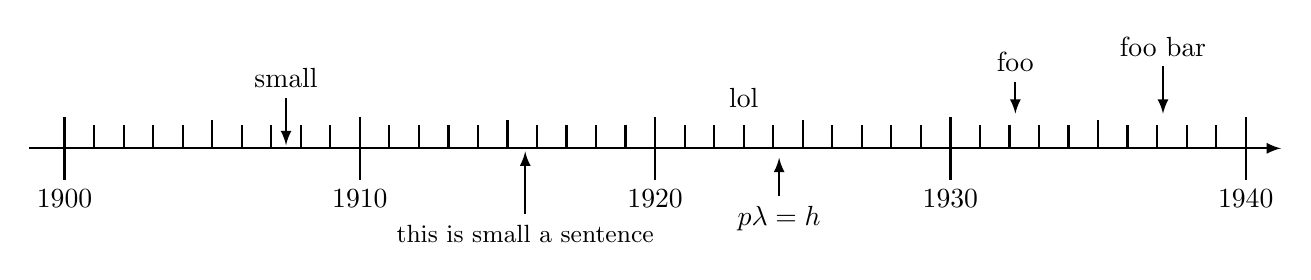
\begin{tikzpicture}[]
  
  % limits
  \newcount\yearOne; \yearOne=1900
  \def\w{15}    % width of axes
  \def\n{4}     % number of decades
  \def\lt{0.40} %  ten tick length
  \def\lf{0.36} % five tick length
  \def\lo{0.30} %  one tick length
  
  % help functions
  \def\yearLabel(#1,#2){\node[above] at ({(#1-\yearOne)*\w/\n/10},\lt) {#2};}
  \def\yearArrowLabel(#1,#2,#3,#4){
    \def\xy{{(#1-\yearOne)*\w/\n/10}}; \pgfmathparse{int(#2*100)};
    \ifnum \pgfmathresult<0
      \def\yyp{{(\lt*(0.90+#2))}}; \def\yyw{{(\yyp-\lt*#3)}}
      \draw[<-,thick,black,align=center] (\xy,\yyp) -- (\xy,\yyw) node[below,black] at (\xy,\yyw) {#4};
    \else
      \def\yyp{{(\lt*(0.10+#2)}}; \def\yyw{{(\yyp+\lt*#3)}}
      \draw[<-,thick,black,align=center] (\xy,\yyp) -- (\xy,\yyw) node[above,black] at (\xy,\yyw) {#4};
    \fi}
  
  % axis
  %\draw[thick] (0,0) -- (\w,0);
  \draw[->,thick] (-\w*0.03,0) -- (\w*1.03,0);
  
  % ticks
  \foreach \tick in {0,1,...,\n}{
    \def\x{{\tick*\w/\n}}
    \def\year{\the\numexpr \yearOne+\tick*10 \relax}
  	\draw[thick] (\x,\lt) -- (\x,-\lt) % ten tick
	             node[below] {\year};
	
	\ifnum \tick<\n
	  \draw[thick] ({(\x+\w/\n/2)},0) -- ({(\x+\w/\n/2)},\lf); % five tick
      \foreach \ticko in {1,2,3,4,6,7,8,9}{
        \def\xo{{(\x+\ticko*\w/\n/10)}}
  	    \draw[thick] (\xo,0) -- (\xo,\lo);  % one tick
	}\fi
  }
  
  % label
  \yearLabel(1923,lol)
  \yearArrowLabel(1932.2, 1.0,1.0,foo)
  \yearArrowLabel(1937.2, 1.0,1.5,foo bar)
  \yearArrowLabel(1907.5, 0.0,1.5,small)
  \yearArrowLabel(1915.6,-1.0,2.0,\small this is small a sentence)
  \yearArrowLabel(1924.2,-1.2,1.2,$p\lambda=h$)
  
\end{tikzpicture}

\end{document}